\documentclass[tikz,border=5pt]{standalone}
\usepackage{amsmath,amssymb}
\usetikzlibrary{arrows.meta,positioning}
\definecolor{curveblue}{HTML}{245C86}
\definecolor{accent}{HTML}{A65E2E}
\begin{document}
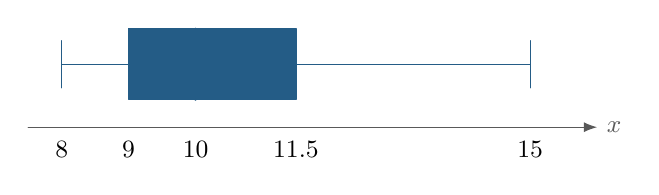
\begin{tikzpicture}[font=\small,>=Latex,line cap=round,line join=round]
\begin{scope}[x=.85cm,y=1cm]
\draw[black!65,->] (7.5,0)--(16,0) node[right]{$x$};
\draw[curveblue] (8,.5)--(8,1.1) (15,.5)--(15,1.1) (8,.8)--(9,.8) (11.5,.8)--(15,.8);
\draw[fill=curveblue!12,curveblue] (9,.35) rectangle (11.5,1.25);\draw[curveblue,thick] (10,.35)--(10,1.25);
\node[below] at (8.00000,-0.06000) {$8$};
\node[below] at (9.00000,-0.06000) {$9$};
\node[below] at (10.00000,-0.06000) {$10$};
\node[below] at (11.50000,-0.06000) {$11.5$};
\node[below] at (15.00000,-0.06000) {$15$};
\end{scope}
\end{tikzpicture}
\end{document}
